\section{Efectos Biológicos del Campo Magnético}

Es necesario evaluar los riesgos y peligros potenciales por la exposición a la Resonancia Magnética (RM), tanto los efectos biológicos directos producidos por la exposición del organismo a la magnetización, como los efectos indirectos producidos por accidentes durante el proceso. Con el fin de discutir válidamente estos riesgos, se deben considerar todos los componentes del proceso de imágenes por RM. Estos componentes incluyen: a) el campo magnético principal, también conocido como el campo magnético estático (\Bzero); b) el campo magnético del gradiente; y c) los campos creados por el transmisor de radiofrecuencia y las bobinas receptoras. Cada uno de estos componentes será descrito a continuación, enfatizando sus repercusiones en los sistemas biológicos.

\subsection{Campo magnético estático (\Bzero)}

Es importante tener en cuenta que el campo magnético estático es el responsable de la alineación de los protones de hidrógeno para la posterior obtención de las imágenes por RM. Los equipos de RM generalmente tienen un campo magnético horizontal.  Para comprender completamente los efectos biológicos de la exposición a la RM, es necesario entender la física de los fenómenos magnéticos, la cual puede ser descrita en términos de física clásica.   Los magnetos permanentes y el flujo de corriente directa a través de materiales conductores, como es el caso de la corriente eléctrica, generan la manifestación de ciertas propiedades físicas de la materia que se encuentra próxima a estos materiales; estas propiedades son bien conocidas y se pueden observar, por ejemplo, cuando la limadura de hierro es expuesta a estos campos, produciendo una orientación en dirección al mismo. Esta propiedad originada por los magnetos o el flujo de corriente directa es denominada campo magnético. El campo magnético es representado por \Bzero y es una magnitud vectorial, es decir, en un punto del espacio donde existe campo magnético se puede definir el valor del campo, su dirección y su sentido (Figura \ref{fig:seguridad_bcero}). 

\begin{figure}[htb]
\begin{figg}
   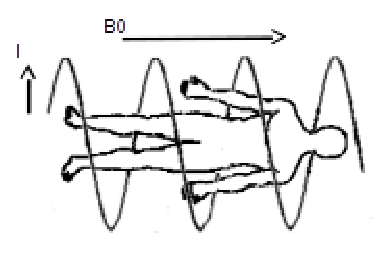
\includegraphics[width=0.7\textwidth]{seguridad_bcero}
   \caption{Campo Magnético creado por un conductor de forma helicoide: I representa la corriente continua que circula a lo largo de conductor y B0 representa el campo magnético generado. }
 \label{fig:seguridad_bcero}
 \end{figg}
\end{figure}




El valor de \Bzero es expresado en unidades de inducción magnética que, para RM, son el Tesla (T) y el Gauss. Un campo magnético es una magnitud vectorial con una dirección (como se mencionó anteriormente), que circula alrededor de un sistema de corriente que lo produce y cuya magnitud decrementa con el cuadrado de la distancia del sistema de corriente. Cuando un material que contiene protones de Hidrógeno es colocado dentro de un campo magnético, el momento magnético de estos comienza a precesar alrededor del campo estático. La frecuencia de precesión depende de la densidad de flujo magnético local y el núcleo en cuestión  (para el caso del protón del núcleo de Hidrógeno presente en la molécula de agua, la frecuencia de resonancia es de 42.57 MHz/T, conocida como la frecuencia de Larmour). Entendiendo el mecanismo mediante el cual ocurre el fenómeno de RM,  ahora se pueden abordar los efectos sobre los sistemas biológicos producidos por la exposición a campos magnéticos.

\subsection{Efectos biológicos}

La introducción de la tecnología de RM a los contextos clínicos desde 1980 ha provocado un incremento sustancial en la exposición del hombre a potentes campos magnéticos estáticos \cite{Schenck_2000}. La mayoría de los sistemas de RM en uso, hoy en día, operan con campos magnéticos estáticos que van desde 0.2 hasta 3 T. En el marco de la investigación, se utilizan campos magnéticos excepcionalmente potentes de hasta 8 T. Según las últimas directrices de la \emph{Food and Drug Administration} (FDA), la utilización clínica de campos magnéticos estáticos de 8.0 T se considera de ``bajo riesgo'' para los pacientes; sin embargo, la exposición de los sujetos de investigación a campos mayores a 8 T requiere la aprobación de un comité de revisión institucional y el consentimiento informado de los sujetos \cite{Shellock_2000}.

Es importante evaluar los efectos fisiológicos que la exposición a la RM podría producir, tales como enlentecimiento en la velocidad de conducción nerviosa, perturbaciones en la electrofisiología normal y efectos sobre la dinámica de los fluidos \cite{Magin_Liburdy_Persson_1992,HealthProtectionAgency_2008};algunos de estos fenómenos se resumen a continuación. 

\subsubsection{Efectos sobre la velocidad de conducción nerviosa}
El argumento teórico de una posible disminución en la velocidad de conducción de los nervios por la exposición a campos magnéticos, se basa en que los campos magnéticos actúan sobre las corrientes iónicas de la misma manera que actúan sobre una carga eléctrica moviéndose en un campo: 
\begin{equation}
 F = q(\nu \cdot B_0)
 \label{eq_F}
\end{equation}
donde $q$ es la carga, $\nu$ es la velocidad y \Bzero es el campo magnético. Esta fuerza causa una distorsión que es perpendicular tanto al campo magnético como a la dirección original del movimiento iónico. Un campo magnético perpendicular a los circuitos de corriente asociados con la propagación a lo largo del nervio podría resultar en una distorsión de estos mismos circuitos y consecuentemente en una disminución de la velocidad de la corriente. De manera teórica, Wikswo y Barach (1980) \cite{Wikswo_Barach_1980} demostraron que se requiere de una potencia de 24 T para reducir la velocidad de conducción del potencial de acción en un 10\%; sin embargo, otros estudios no han reportado cambios en la conducción nerviosa en equipos de 2 a 9 T. Una posible explicación a esto es que la velocidad de conducción podría cambiar debido a la falta de un adecuado control de la temperatura, ya que un cambio de 0.2\degrees \xspace podría causar cerca del 2\% de cambio en la conducción de la velocidad.

Efectos sobre el Electrocardiograma. Un potencial eléctrico puede ser producido por un conductor en movimiento tal como el flujo sanguíneo, el pulso cardiaco o la respiración de los pulmones en un campo magnético. El potencial eléctrico inducido por este movimiento produce una señal superpuesta en el electrocardiograma normal, la cual incrementa con la fuerza del campo:
\begin{equation}
 E=\nu \cdot B_0 \cdot d
\end{equation}
para un flujo que se conduce de manera perpendicular al campo magnético, donde $E$ es el potencial eléctrico y $d$ es el diámetro del vaso. La magnitud del campo $E$ asociado a este cambio en el potencial es mucho menor que el necesario para producir una excitación eléctrica del corazón, lo que se concluye teóricamente, ya que, a 10 T, el campo $E$ en la aorta es 10 veces menor que el campo $E$ teórico necesario para una excitación eléctrica cardiaca.

\subsubsection{Efectos sobre el Electroencefalograma}
Reportes en la literatura sobre los efectos del campo magnético en las ondas cerebrales en diversos experimentos usando electrodos implantados en el cerebro de modelos animales  han reportado efectos asociados con artefactos producidos por el movimiento de los electrodos dentro del campo magnético, no así, efectos fisiológicos.

\subsubsection{Efecto de Frenado en el Flujo de Conductores} 
Considerando un tubo de sangre que fluye a una velocidad $\nu$ perpendicular al campo magnético (\Bzero) y que, como ya se mencionó, se tiene que una fuerza $F$ sobre los conductores es dada por la ecuación \ref{eq_F}:
La corriente de iones asociada con esta fuerza está relacionada a la conductividad. Esta corriente es también perpendicular al campo magnético  y al flujo; es el resultado de la interacción de esta corriente y el campo magnético estático y otra fuerza que se encuentra en dirección opuesta a la velocidad de la sangre. Sin embargo, cálculos teóricos acerca de la dinámica de este efecto, muestran que este no es significativo para producir cambios en la dinámica circulatoria en humanos. Lo cual es congruente con la ausencia de reportes de efectos significativos en humanos, con excepción de vértigos y nauseas en algunos sujetos a 4 T.

Schenck \cite{Schenck_2000,Schenck_1992} ha llevado a cabo un amplio análisis de los efectos biológicos asociados a la exposición a campos magnéticos estáticos. Con respecto a la exposición a corto plazo (por ejemplo, aquellas exposiciones asociadas con el uso clínico de los sistemas de RM), la información disponible sobre los efectos de los campos magnéticos estáticos en los tejidos biológicos es extensa \cite{Schenck_2000,Schenck_1992,Besson_Foreman_Eastwood_Smith_Ashcroft_1984}. Las investigaciones incluyen estudios sobre las alteraciones en crecimiento y morfología celular, reproducción celular y teratogenicidad, estructura del ADN y expresión genética, desarrollo pre y postnatal, permeabilidad de la barrera hemato-encefálica, actividad nerviosa, función cognitiva y conducta, dinámica cardiovascular, índices hemáticos, regulación de la temperatura, ritmos circadianos, respuesta inmune y otros procesos biológicos. En la mayoría de estos estudios, los autores concluyeron que la exposición a campos magnéticos estáticos no produce efectos biológicos nocivos importantes. Aunque ha habido algunos reportes de los efectos potencialmente perjudiciales de los campos magnéticos estáticos sobre células aisladas o de los organismos, ninguno de estos efectos se han comprobado o establecido de manera concluyente como un hecho científico. Las lesiones producidas por el uso de sistemas de RM son relativamente poco documentadas y se atribuyen principalmente a la presencia accidental o introducción de objetos ferromagnéticos al equipo de RM.

\subsubsection{Objetos ferromagnéticos}
Aparte de los posibles efectos biológicos producidos por la exposición a la RM, hay que tener siempre presentes los riesgos que conlleva esta tecnología en relación a su efecto sobre los objetos metálicos, como ya se mencionó anteriormente.  Es importante definir qué objetos pueden verse afectados por los campos magnéticos y pueden constituir un riesgo potencial al momento de utilizar esta tecnología. De acuerdo con su comportamiento al ser sometidos a campos magnéticos, las sustancias y objetos pueden clasificarse en tres categorías:
\begin{description}
 \item [Paramagnéticas] Son débilmente atraídas hacia la zona de campo magnético más intenso.
 \item [diamagnéticas] Son débilmente repelidas hacia las regiones de menor campo magnético. 
 \item [ferromagnéticas] Son fuertemente atraídas hacia la zona de campo magnético más intenso. 
\end{description}



Si el campo magnético externo es el creado en el interior de un solenoide de valor $B_0 = \mu_0 nl$, al situar dentro del solenoide una sustancia, el campo pasará a tener un valor $B_0 = \mu nl$, donde $\mu$ es la permeabilidad magnética de la sustancia. La permeabilidad de cualquier medio puede expresarse como $\mu = \mu_r \mu_0$ , donde $\mu_r$ es la permeabilidad relativa. Usualmente se define: $\mu_r = 1 + \chi_m$ , donde $\chi_m$ es la susceptibilidad magnética, una magnitud importante para caracterizar el comportamiento magnético de las sustancias.

El \textbf{diamagnetismo} es una forma muy débil de magnetismo que no es permanente y persiste sólo mientras se aplique un campo externo, este es inducido por un cambio en el movimiento orbital de los electrones debido a la aplicación de un campo magnético. La magnitud del momento magnético inducido es extremadamente pequeña y en dirección opuesta al campo aplicado, por ello, $\mu_r$ es menor que la unidad y la susceptibilidad magnética, es negativa; o sea que la magnitud del campo magnético B dentro de un sólido diamagnético es menor que en el vacío. El diamagnetismo produce una susceptibilidad magnética negativa muy débil, del orden de $\chi_m = 10^{-6}$.  Cuando un material diamagnético se coloca entre polos de un electromagneto fuerte, es atraído hacia las regiones donde el campo es débil. El diamagnetismo se encuentra en todos los materiales pero solo puede observarse cuando otros tipos de magnetismo están totalmente ausentes. Esta forma de magnetismo no tiene importancia práctica.

En el caso del \textbf{paramagnetismo} se debe considerar que para algunos materiales sólidos cada átomo posee un momento dipolar permanente en virtud de la cancelación incompleta del spin electrónico y/o de los momentos magnéticos orbitales. En ausencia de un campo magnético externo, las orientaciones de esos momentos magnéticos son al azar, tal que una pieza del material no posee magnetización macroscópica neta. Esos dipolos atómicos son libres para rotar y cuando se alinean en una dirección preferencial por rotación al aplicar un campo externo, resulta el paramagnetismo. Estos dipolos magnéticos actúan individualmente sin interacción mutua entre dipolos adyacentes. Como los dipolos se alinean con el campo externo, actúan en forma sinérgica dando lugar a una $\mu_r$ mayor que la unidad y a una susceptibilidad magnética relativamente pequeña pero positiva. El efecto del paramagnetismo desaparece cuando se elimina el campo magnético aplicado.


Para aquellos materiales que poseen un momento magnético permanente en ausencia de un campo externo y manifiestan magnetizaciones muy largas y permanentes se habla de \textbf{ferromagnetismo}, el cual es presentado por algunos metales de transición, Fe, Co, Ni y algunas tierras raras como el gadolinio (Gd). Cuando se hace incidir un campo magnético sobre una sustancia ferromagnética, se produce un desplazamiento de las paredes de los dominios, de modo que aumenta el número de aquellos cuyo momento magnético está orientado a favor del campo y disminuye el de los demás. Si el campo externo es lo suficientemente intenso, se puede producir, incluso, un giro brusco de los momentos magnéticos de los dominios en la dirección del campo, lo que aumenta la magnetización del material. El imán o material ferromagnético puede mantener durante mucho tiempo esta orientación de sus dominios, aún si desaparece el campo externo.  Estos objetos ferromagnéticos requieren de especial atención en los procedimientos de RM, ya que la forma en la que interactúan con los campos magnéticos puede convertirlos en proyectiles, produciendo severos daños en los pacientes que ingresan a los equipos de RM. Por ejemplo, pequeños objetos ferromagnéticos, como clips y pasadores para el cabello, pueden alcanzar una velocidad de 64 km/hr cuando son introducidos en un campo magnético de 1.5 T. 

Muchos de los materiales de cirugía, como pinzas, tijeras y otros implementos de acero inoxidable o sustancias ferromagnéticas, se ven atraídos por el campo magnético generado en la RM. Entre otros objetos ferromagnéticos se pueden identificar implantes, dispositivos y otros materiales colocados en algunos pacientes que producen los mismos efectos que cualquier otro objeto ferromagnético. Los principales efectos incluyen: la generación de proyectiles, deformaciones de los implantes y dispositivos por torsión de los metales, calentamiento y subsecuentes quemaduras, y artefactos en la imagen por RM. Antes de permitir el acceso de los participantes o pacientes al entorno de RM se debe realizar una selección cuidadosa para determinar la presencia de implantes, dispositivos u objetos que puedan representar peligros o riesgos. Una vez identificados, se debe decidir si es aceptable que el participante o paciente ingrese al entorno de RM o se someta a un procedimiento de RM. En los apartados siguientes se abordará con mayor detalle las reglas de compatibilidad y las restricciones en cuanto al uso de ciertos materiales.

\subsection{Campo magnético del gradiente}
Todos los sistemas de RM están equipados con un conjunto de bobinas conocido como bobinas de gradiente. La función de los gradientes es proporcionar una variación en la fuerza del campo magnético encendiendo y apagando  pulsos de gradiente entre los pulsos de excitación de radiofrecuencia. El propósito de estos gradientes es el de codificar espacialmente la información contenida en la señal de radiofrecuencia producida por la caída y relajación de los spins; sin embargo, al hacerlo, se crea un campo magnético variable en el tiempo. Esta variación del campo magnético en el tiempo puede inducir corrientes eléctricas en los circuitos biológicos y, si ésta fuese importante, podría causar excitación de las células musculares o nerviosas, fibrilaciones, aumento de osmolaridad cerebral y alteración de la remodelación ósea.

Es importante considerar que si la corriente inducida es suficiente, podría generarse un potencial de acción en los tejidos excitables. Para la estimación de la corriente inducida se debe tomar en cuenta que la densidad de corriente inducida ($J$) depende de la conductividad eléctrica del medio ($\sigma$), de las condiciones geométricas del circuito (Superficie: $S$ y Longitud del conductor: $L$), de la magnitud de la variación del campo magnético ($dB/dt$) y de la dirección del campo magnético respecto a la superficie:
\begin{equation}
  J = \sigma \cdot S/L \cdot dB/dt
\end{equation}

Si consideramos que la densidad de corriente para crear un potencial de acción en un nervio es de 300 $\mu$A/$cm^2$ \cite{Budinger_1983}, tenemos que, para obtener la magnitud de la variación del campo magnético que induciría el potencial de acción, sólo se despeja la formula considerando valores conocidos respecto a $\sigma$ y $S/L$ del conductor, dada por el radio considerando un conductor circular. De esta manera, se obtendría la magnitud del gradiente máximo. La FDA ha establecido como valores máximos aconsejables: variaciones de campo magnético del orden de los 20 T/s para pulsos mayores de 120 $\mu$s, o 200 T/s para pulsos de amplitud menor de 12 $\mu$s. Además se debe cuidar la colocación de los pacientes en las exploraciones dentro del escáner, ya que pueden formarse circuitos en el cuerpo o body loops, los cuales pueden inducir corrientes; para ello, se debe instruir al paciente para que no cruce los brazos o las piernas durante la exploración, también pueden separarse estos puntos de contacto mediante material no conductor.

Como ya se mencionó anteriormente, durante los procedimientos de RM, el gradiente de campo magnético puede estimular los nervios o los músculos mediante la inducción de campos eléctricos en los pacientes. El tema ha sido ampliamente revisado \cite{Nyenhuis_Bourland_Schaefer_1997,Bourland_Nyenhuis_Schaefer_1999}. Las interacciones entre gradiente de campo magnético y tejido biológico dependen de una variedad de factores, incluyendo la frecuencia del campo principal, la densidad de flujo máximo, la densidad media de flujo, la presencia de frecuencias armónicas, las características de forma de onda de la señal, la polaridad de la señal, la distribución de corriente en el cuerpo, las propiedades eléctricas y la sensibilidad de la membrana celular. Dos de los efectos biológicos mejor identificados en relación a los cambios de gradientes en el campo magnético son la estimulación del nervio periférico y el ruido acústico; a continuación se describirán algunas de sus características.

\subsubsection{Estimulación nerviosa periférica}
La aplicación de gradientes de campo magnético puede inducir una corriente en materiales conductores, incluyendo los nervios y el tejido muscular. La corriente inducida es mayor en los tejidos periféricos y se pueden producir sensaciones leves en la piel y contracciones musculares involuntarias. Estas sensaciones pueden escalar a sensaciones dolorosas o desagradables si se incrementa la intensidad del gradiente de campo magnético; al escanear, se pueden inducir corrientes que influyan en la función cardiaca y, en casos extremos, causen fibrilación ventricular. Los estudios llevados a cabo en los participantes durante investigación, indican que los sitios anatómicos donde se produce la estimulación de nervios periféricos por efecto de los gradientes de campo magnético, varían en función de la activación de un gradiente específico (es decir en el gradiente $x$, $y$, $z$) (Tabla \ref{tab_seguridad}). Por lo general, los sitios de estimulación del nervio periférico se han encontrado en las prominencias óseas; ya que el hueso es menos conductor que el tejido circundante, las densidades de corriente pueden aumentar en regiones estrechas de tejido entre el hueso y la piel, lo cual reduce los umbrales de estimulación nerviosa más de lo esperado. Los individuos sometidos a RM deben ser instruidos para reportar cualquier sensación al operador del escáner, para llevar a cabo la acción pertinente \cite{Kangarlu_Robitaille_2000,HealthProtectionAgency_2008}. 


\begin{table}[hbtp]
\centering
\caption{Sitios de estimulación según el gradiente aplicado (Medical College of Wisconsin 2009)}
\label{tab_seguridad}
\begin{tabular}{@{}ll@{}}
\toprule
\textbf{Sitios de Estimulación del Nervio Periférico} & \textbf{Gradiente}   \\ \midrule
Puente de la nariz                           & $x$         \\
Hombros                                      & $y$         \\
Escápula                                     & $y$,$z$     \\
Porción proximal de los brazos               & $y$         \\
Espalda alta                                 & $y$,$z$     \\
Tórax                                        & $z$         \\
Porción izquierda del tórax                  & $x$         \\
Porción derecha del tórax                    & $y$         \\
Xifoides                                     & $z$         \\
Abdomen                                      & $z$         \\
Cresta iliaca                                & $x$,$y$,$z$ \\
Espalda baja                                 & $x$, $z$    \\
Cadera                                       & $y$         \\
Nalgas                                       & $x$         \\
Muslo izquierdo                              & $x$         \\
Manos                                        & $y$         \\ \bottomrule
\end{tabular}
\end{table}


\subsection{Ruido acústico}
Otra de las consecuencias del encendido y apagado de los gradientes es que, en presencia de un campo magnético estático, las corrientes en las bobinas de gradiente generan fuerzas que implican vibraciones con sus consecuentes ruidos, los cuales pueden llegar a ser de alta intensidad \cite{Shellock_2000}. La frecuencia y la tonalidad dependen de muchos factores, entre ellos el diseño de aparato y la secuencia utilizada \cite{Miyati_Banno_Fujita_Mase_Narita_Imazawa_Ohba_1999}. Los problemas asociados con el ruido acústico para los pacientes o participantes y el personal incluyen: simple irritación, dificultades en la comunicación verbal, incremento de la ansiedad, pérdida de audición temporal y, posiblemente, deterioro permanente de la audición \cite{McJuryPhD_ShellockPhD_2000,Hurwitz_Lane_Bell_Brant-Zawadzki_1989}. El ruido acústico puede representar un peligro, en particular para grupos específicos de pacientes que están en mayor riesgo. Los pacientes con trastornos psiquiátricos, ancianos, y niños pueden presentar sensaciones de confusión o una mayor experiencia de ansiedad \cite{Quirk_Letendre_Ciottone_Lingley}. Los pacientes sedados pueden experimentar malestar general debido a los altos niveles de ruido. Ciertos medicamentos, conocidos por aumentar la sensibilidad auditiva, pueden producir mayores sensaciones de malestar \cite{Laurell_1992}. Los recién nacidos con inmadurez en el desarrollo anatómico pueden tener una reacción mayor ante el ruido acústico \cite{Philbin_Taber_Hayman_1996}.

Las variaciones del ruido acústico relacionadas con RM ocurren cuando se realizan modificaciones en la salida de gradiente (incremento del tiempo o de la amplitud) y también se asocia con los distintos parámetros de RM \cite{McJuryPhD_ShellockPhD_2000,Counter_2000,Cho_Park_Kim_Chung_Chung_Chung_Moon_Yi_Sin_Wong_1997}. El incremento en los niveles de ruido, tono y frecuencia se debe principalmente a una reducción en los tiempos de repetición y de eco. Las características físicas del equipo (especialmente la presencia o ausencia de aislamiento especial del sonido y el material con el que se construyeron las bobinas de gradiente y estructuras de apoyo) también influyen en la transmisión de ruido acústico y su percepción por los pacientes o participantes \cite{Philbin_Taber_Hayman_1996}.

La presencia y tamaño del paciente también afecta el nivel de ruido acústico. Se ha informado un incremento en el ruido acústico cuando el paciente o participante se encuentra dentro del escáner, este fenómeno se puede deber a la doble presión que se genera por la cercanía de un objeto, de tal manera que las ondas del sonido se reflejan y sincronizan su fase. Las características del ruido también presentan dependencia del espacio, por ejemplo, se ha descubierto que los niveles varían hasta en 10 dB en función de la posición del paciente a lo largo del diámetro del magneto \cite{Hedeen_Edelstein_1997}.

Los niveles de ruido relacionados con la RM han sido medidos durante diferentes secuencias de pulsos para sistemas de RM que van desde los 0.2 hasta los 4.7 T \cite{Counter_2000,Shellock_2000}. Estudios recientes han demostrado que las secuencias de pulsos de gradiente de eco rápidos, spin-eco y secuencias eco-planares producen un mayor nivel de ruido \cite{Price_DeWilde_Papadaki_Curran_Kitney_2001,McJuryPhD_ShellockPhD_2000}. La FDA indica que los límites permisibles de ruido acústico relacionado con RM se encuentran por debajo del nivel establecido según las regulaciones federales o los estándares propuestos por otras organizaciones. Si el ruido acústico no se encuentra por debajo de estos niveles, el fabricante debe recomendar las medidas pertinentes para la reducción del ruido percibido por el individuo. El pico de ruido acústico de 140 dB es el límite superior; sin embargo, las instrucciones para el uso del equipo deben indicar al operador que se proporcione protección para los oídos a los pacientes o participantes cuando se opere en niveles por arriba de los 99 dB \cite{Shellock_2000}.

En general, si se siguen las reglas establecidas por los organismos reguladores para el control del ruido acústico relacionado con la RM, los procedimientos no suelen ser problemáticos debido a los períodos exposición de tiempo relativamente cortos.




\section{Medidas de prevención de accidentes}

\subsection{Evaluación Clínica}
Los individuos que van a ser expuestos a entornos de RM, ya sea con fines clínicos o de investigación, deben ser evaluados para conocer su condición médica y determinar si existen riesgos para que puedan ingresar a RM; debe considerarse que no tengan problemas que puedan impedir que se mantengan acostados o permanezcan quietos durante largos períodos de tiempo. Aquellos pacientes que requieren mantenerse durante medicación continua a través de dispositivos externos o internos deben ser excluidos como candidatos a estudios de RM; aquellos quienes no entienden las instrucciones o no pueden cooperar con el personal encargado del equipo de RM para asegurar el éxito del estudio deben ser considerados cuidadosamente. Los individuos que portan algún dispositivo o implemento médico de manera permanente o cualquier otro objeto ferromagnético o con características ferromagnéticas deben ser excluidos o evaluados cuidadosamente. En cualquier caso, todos los individuos deben ser evaluados muy rigurosamente para garantizar la seguridad de los implicados y la efectividad del estudio. A continuación se describen algunos procedimientos y aspectos a tomar en cuenta a la hora de considerar a un candidato para RM.

\subsubsection{Formulario de evaluación preliminar}
Antes del ingreso del paciente a la sala de exploración de RM, se debe llevar a cabo una serie de pasos que garanticen la seguridad del mismo; estos se pueden facilitar a través del uso de un cuestionario de escrutinio para detectar riesgos de exploración del paciente en RM, en las Figuras \ref{fig:seguridad_formularioA} y \ref{fig:seguridad_formularioB} se muestra un ejemplo de la información que debe contener dicho cuestionario.



\begin{figure}[htb]
\begin{figg}
   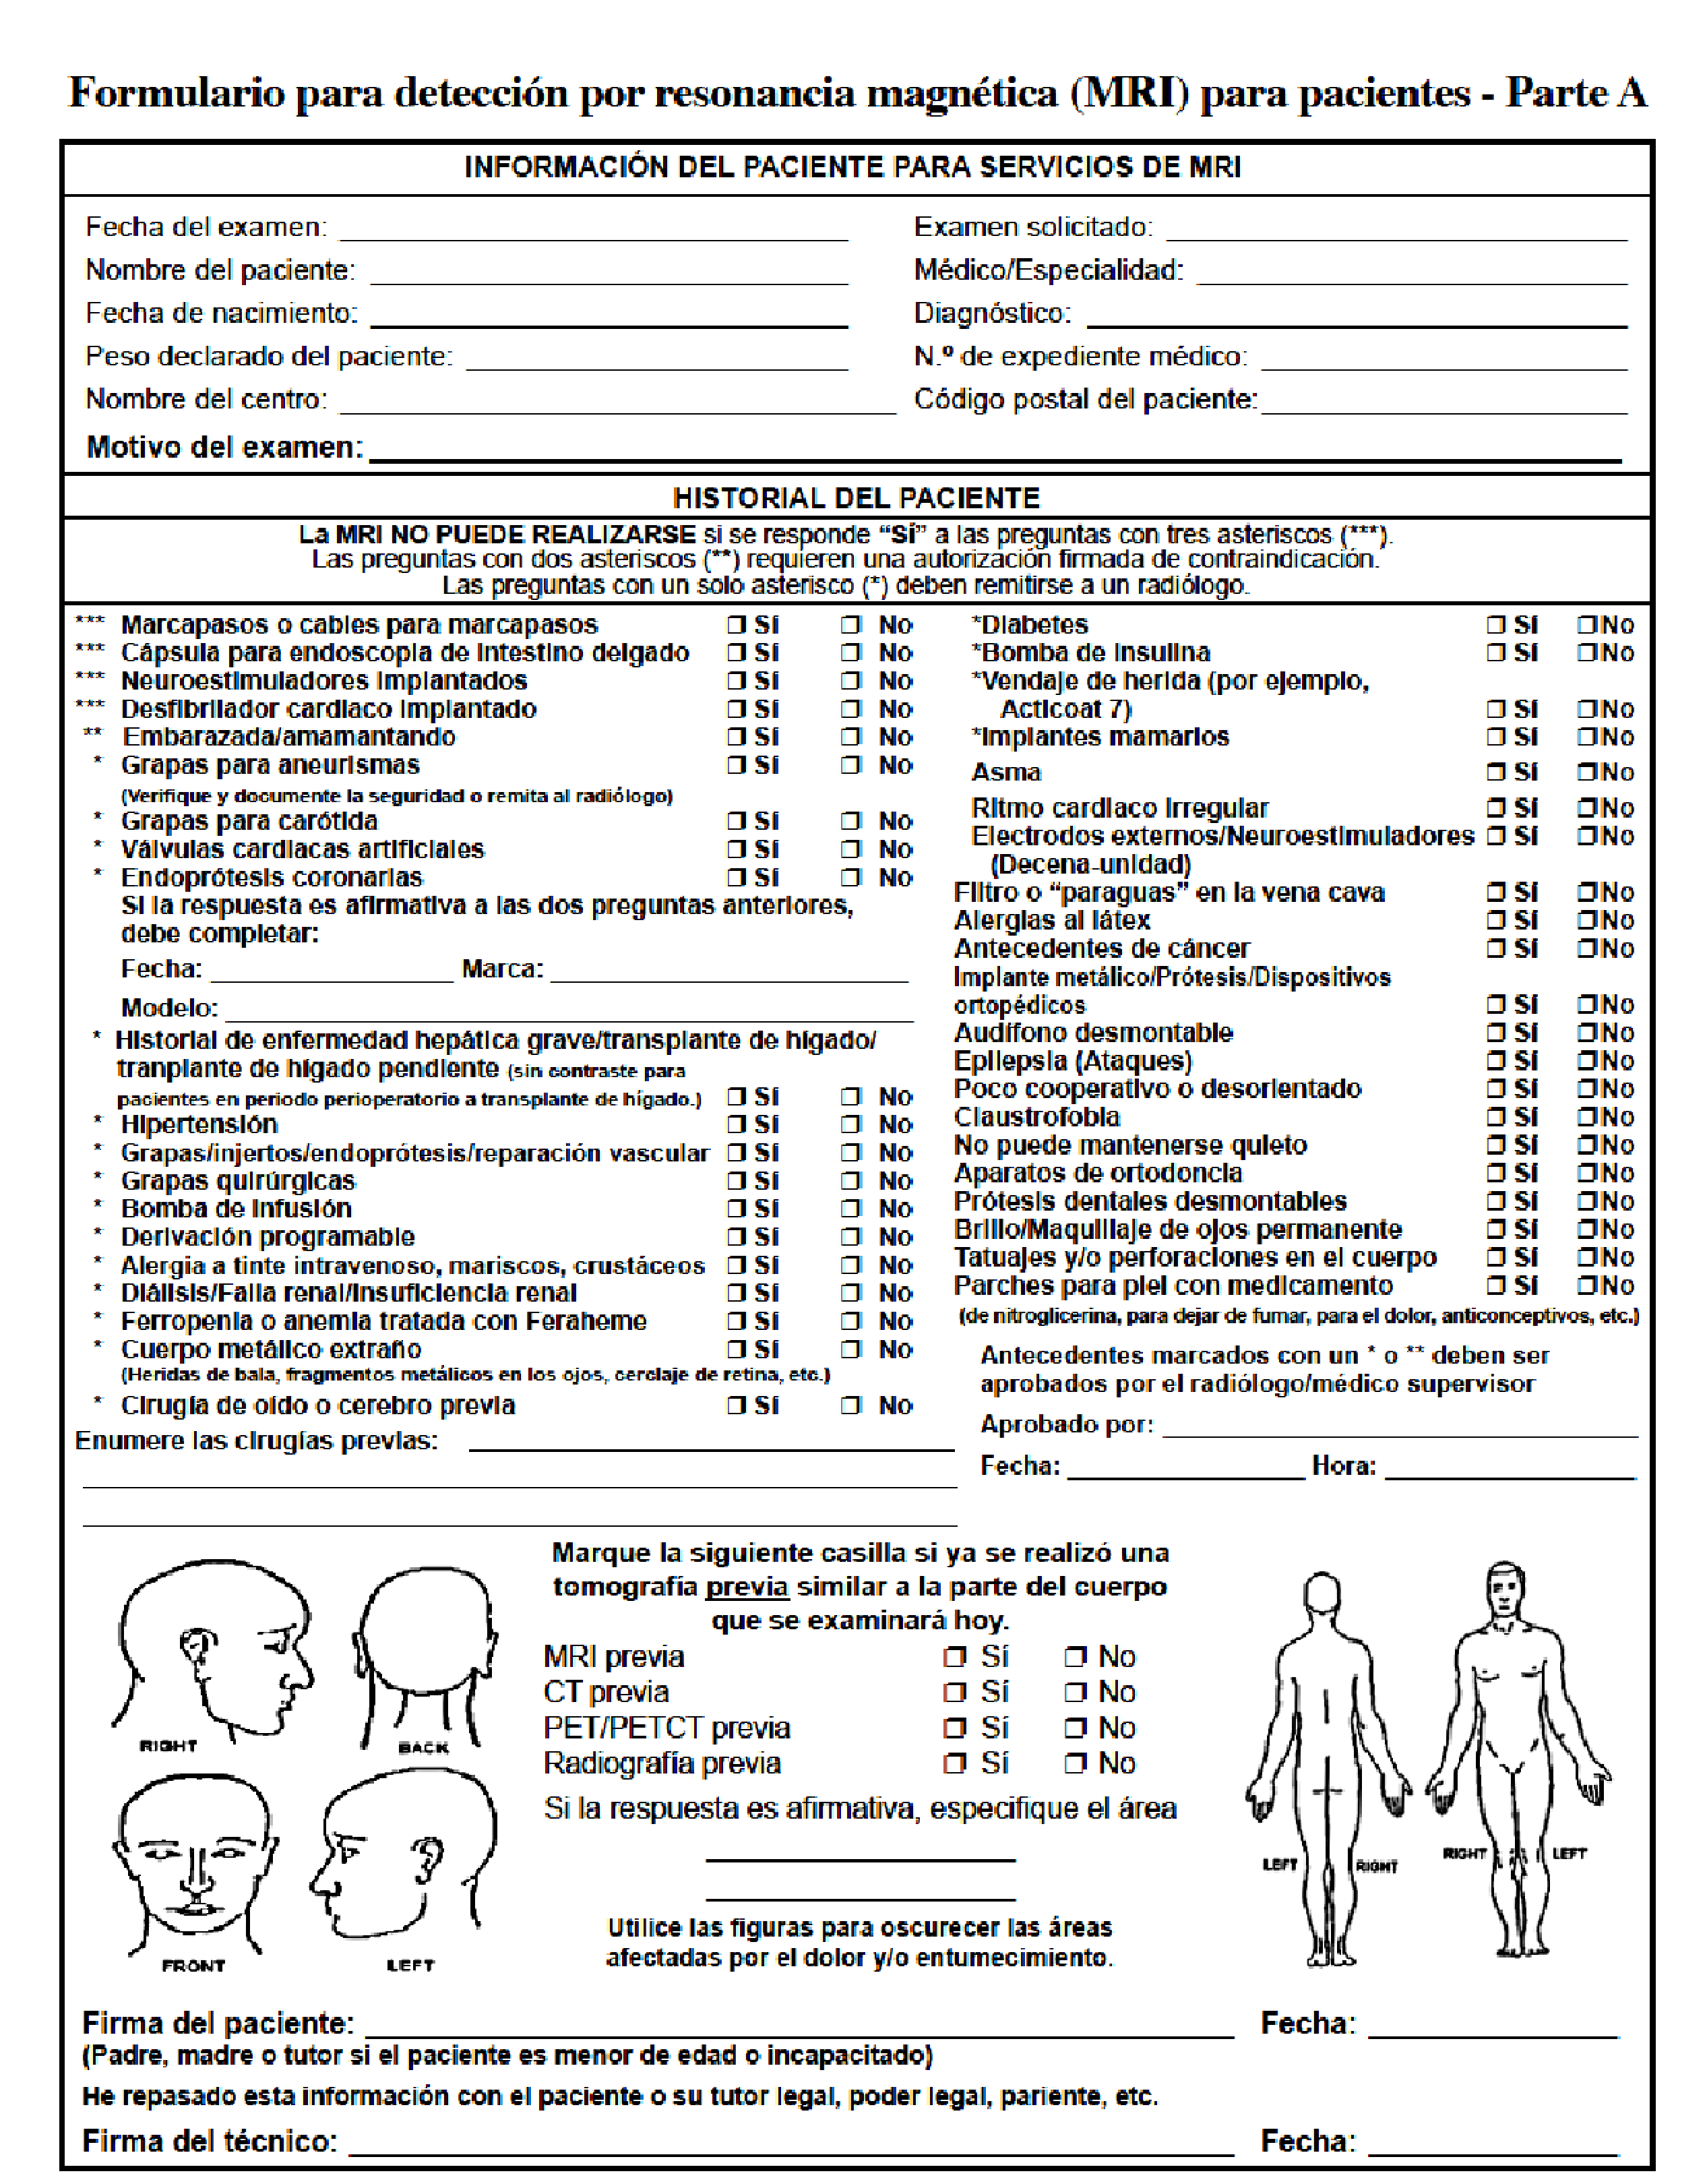
\includegraphics[width=0.7\textwidth]{seguridad_formularioA}
   \caption{Formulario de detección por Resonancia Magnética para pacientes (anverso). Tomado de Day Kimbal Healthcare. }
 \label{fig:seguridad_formularioA}
 \end{figg}
\end{figure}

\begin{figure}[htb]
\begin{figg}
   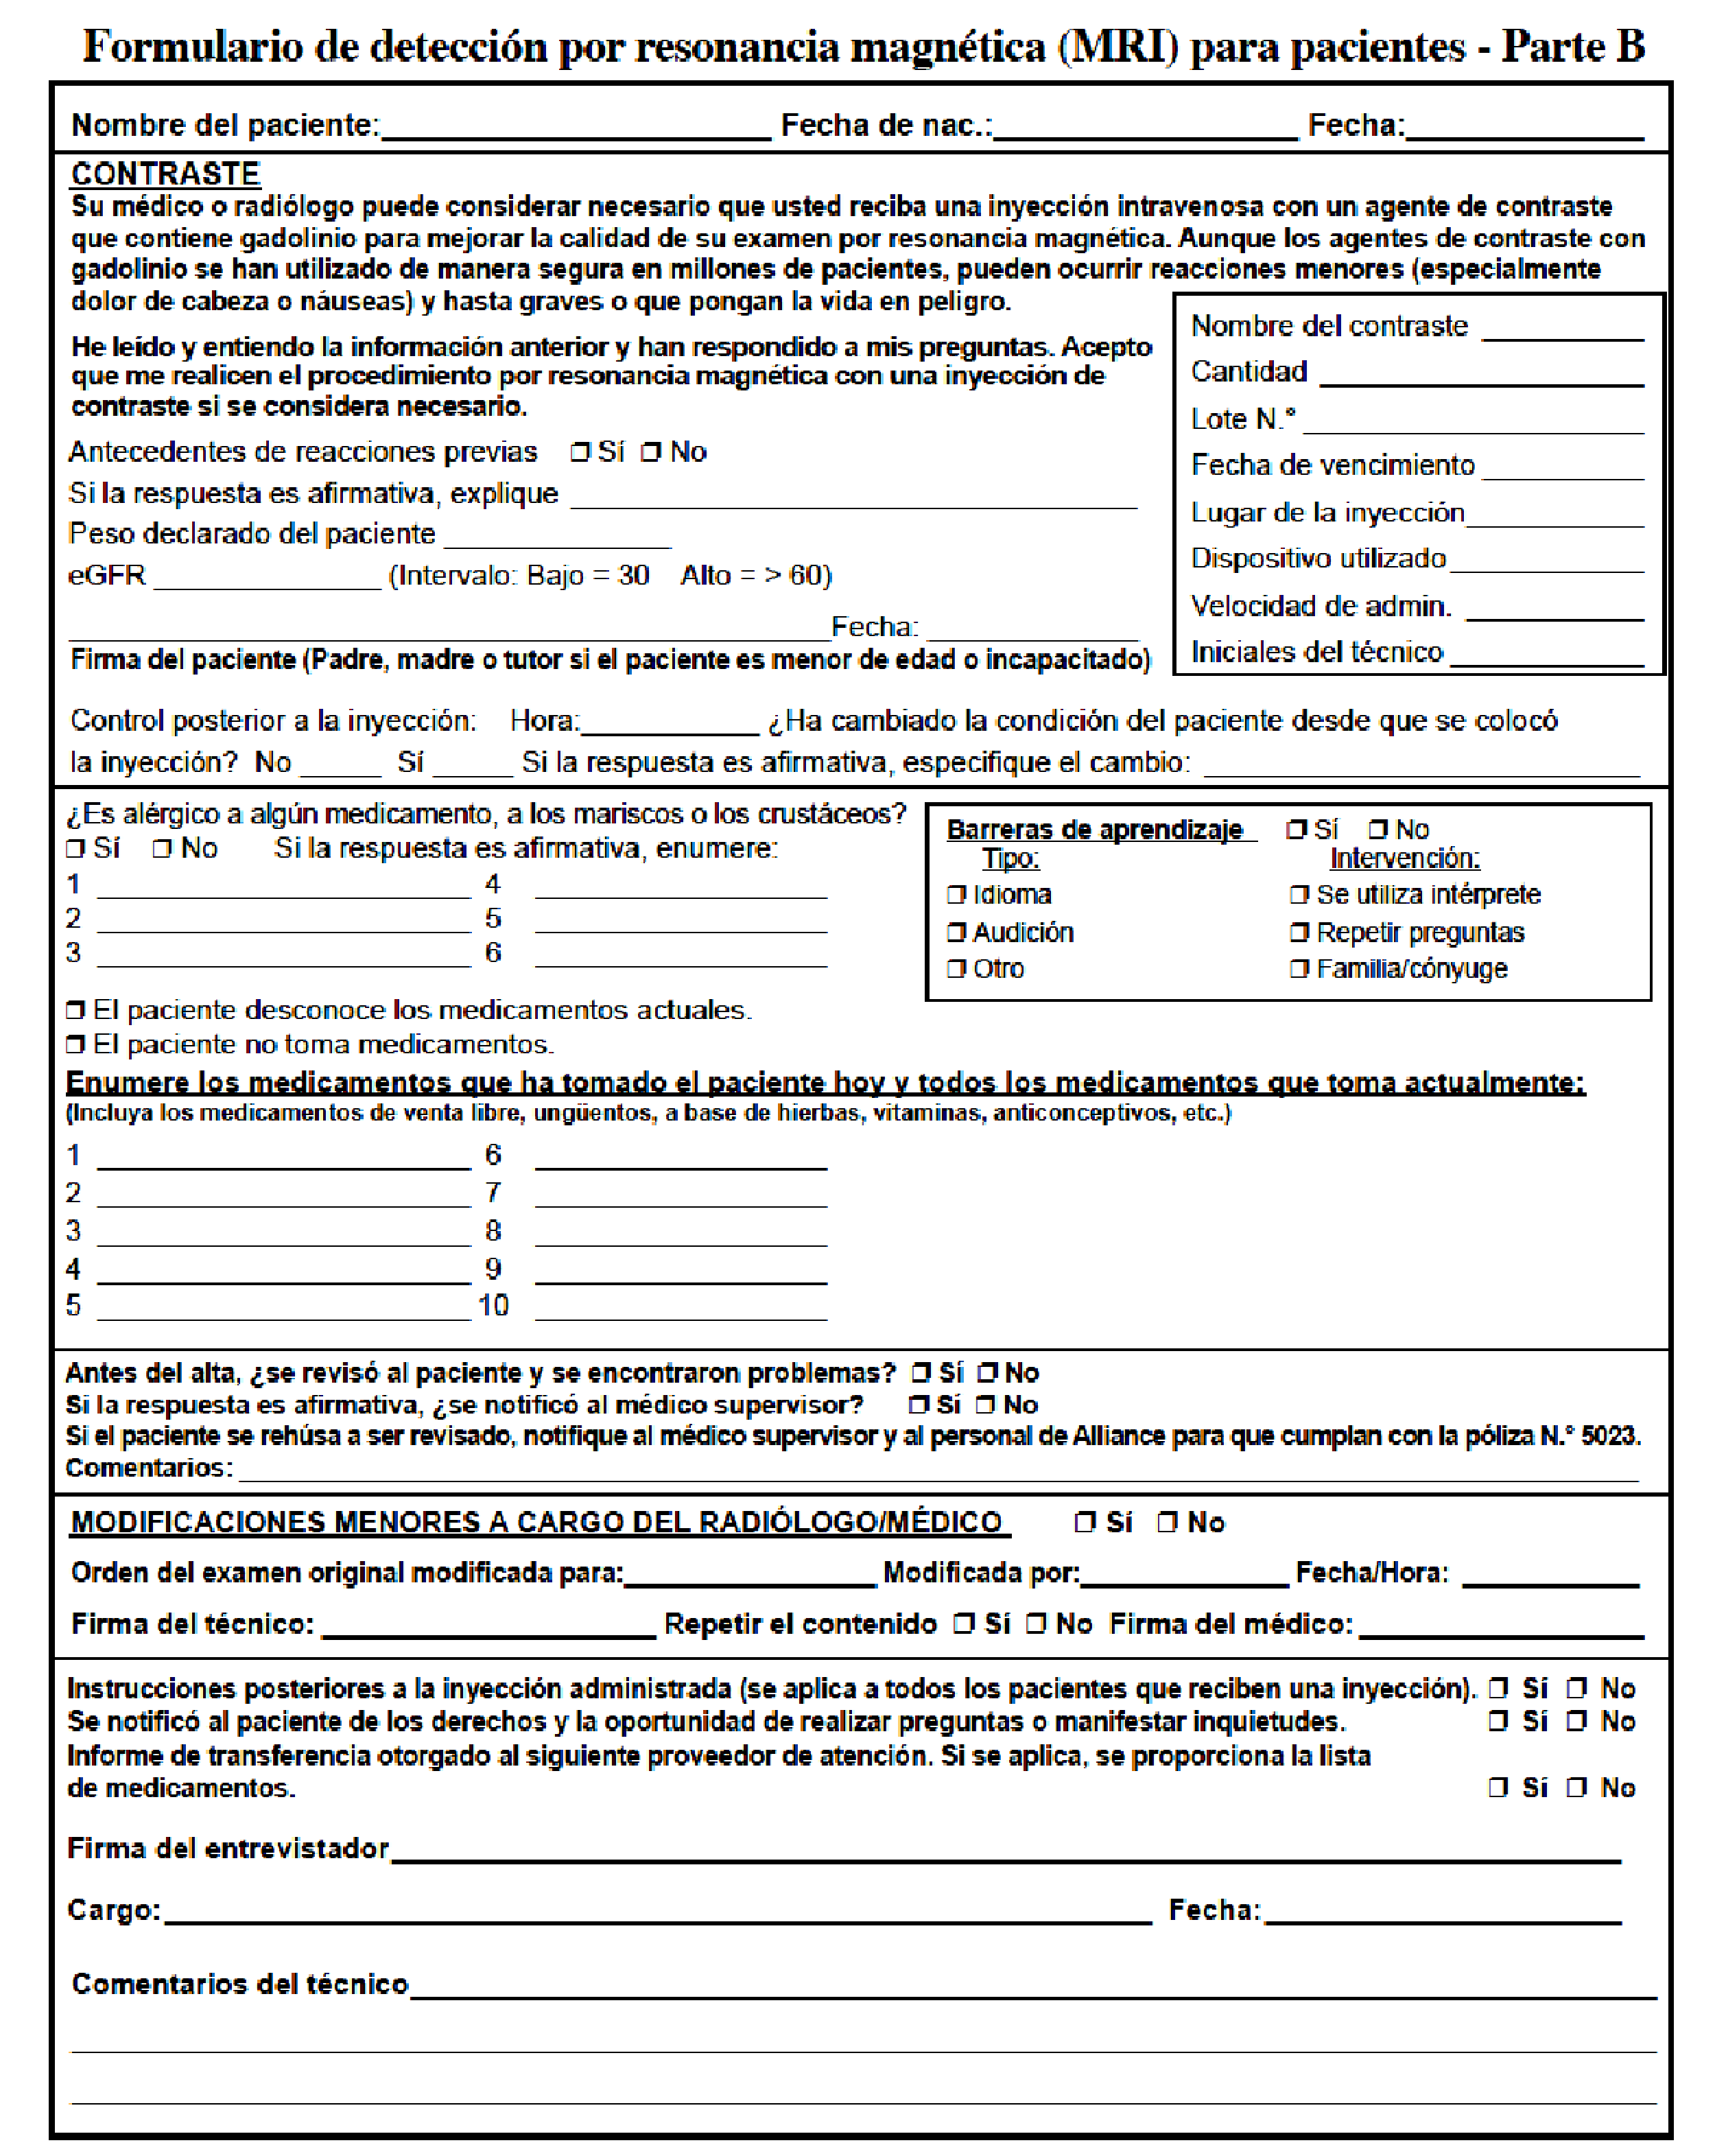
\includegraphics[width=0.7\textwidth]{seguridad_formularioB}
   \caption{Formulario de detección por Resonancia Magnética para pacientes (reverso). Tomado de Day Kimbal Healthcare. }
 \label{fig:seguridad_formularioB}
 \end{figg}
\end{figure}



Los pasos siguientes, que incluyen el uso del formulario, deben de llevarse a cabo antes de iniciar el estudio dentro de la sala de RM: 

\begin{enumerate}
\item Interrogar al paciente sobre posibles implantes metálicos internos y externos al recibirle y antes de entrar en la sala exploración, estableciendo, así, diferentes filtros de seguridad.
\item En caso de duda sobre la compatibilidad de un implante con el equipo de RM, realizar la exploración sólo hasta tener la documentación necesaria sobre el objeto.
\item Retirar audífonos y dentaduras postizas.
\item Retirar materiales metálicos que lleve el paciente externamente (reloj, cadenas, anillos, etc.) y tener la misma conducta para el personal médico, acompañantes, y todo aquel que vaya ingresar a la sala del escáner.
\item Atención al uso de aparatos de reanimación como desfibriladores, tanques de oxígeno, etc., no utilizarlos nunca dentro de la sala de exploración (salvo que exista compatibilidad con RM).
\item Verificar que los pacientes no lleven maquillaje, en caso de que así sea retirárselo. Se debe prestar especial atención a pacientes con tatuajes o con maquillaje permanente, dando instrucciones al individuo para que avise del calentamiento de esa zona y, en el caso de que esto sucediese, retirarlo inmediatamente.
\end{enumerate}



\subsubsection{Compatibilidad con RM}
En 1997, la FDA  y el \emph{Center for Devices and Radiological Health}, crearon dos categorías para el uso de objetos e implementos en los entornos de RM, estos son: RM Seguro y RM Compatible. RM Seguro: aquellos objetos, implantes o dispositivos que cuando son usados en entornos de RM han demostrado no  representar un riesgo adicional para el participante o paciente, aunque pueden afectar la calidad de los datos adquiridos. RM Compatible: aquellos objetos que, aparte de haberse comprobado que son seguros en entornos de RM, cuando son usados tampoco afectan la calidad de los datos que se adquieren. Tanto en los materiales considerados seguros como los materiales considerados compatibles debe especificarse las condiciones en que el material ha sido probado, ya que un material puede considerarse seguro o compatible bajo determinadas condiciones y no en otras condiciones. Sin embargo, estos términos han sido debatidos ya que existe cierta ambigüedad en la práctica. 

Para tener una mayor claridad y certeza de la seguridad de los individuos en entornos de RM la \emph{American Society for Testing and Materials} (ASTM) introdujo en 2005 tres categorías: RM Seguro, RM Condicional y RM No seguro. \textbf{RM Seguro} es aquel material que no representa ningún peligro conocido en todos los entornos de RM. Entre los materiales se incluyen no conductores, objetos no metálicos y no magnéticos. \textbf{RM Condicional} son aquellos objetos en los que no ha sido demostrada su peligrosidad en entornos de RM bajo condiciones específicas, por ello se deben definir y considerar las condiciones del campo magnético para determinar su seguridad. \textbf{RM No seguro} son aquellos objetos cuya peligrosidad es conocida en todos los entornos de RM, como son los objetos ferromagnéticos (Figura \ref{fig:seguridad_simbolos}).



\begin{figure}[htb]
\begin{figg}
   
\includegraphics[width=0.7\textwidth]{seguridad_simbolos}
   \caption{Rótulos indicativos de la compatibilidad de los materiales en entornos magnéticos; de izquierda a derecha RM seguro, RM condicional y RM no-seguro.}
 \label{fig:seguridad_simbolos}
 \end{figg}
\end{figure}






Todo el equipo, usado tanto para fines de investigación como clínicos dentro de entornos de RM incluyendo proyectores, estimuladores y demás aparatos, debe ser probado previamente para verificar su seguridad en espacios magnéticos antes de entrar a alguno. Es responsabilidad del técnico o investigador, nunca tener equipo dentro de la habitación de RM sin haberlo probado previamente para verificar su atracción magnética; se recomienda tener a la mano, fuera del área de RM, un magneto para verificar que los objetos que se introducen al entorno no sean ferromagnéticos. Del mismo modo, se debe tener cuidado en hacer un minucioso escrutinio del participante o paciente para verificar que se encuentra en condiciones de ingresar a las sala de RM. El equipo que opera en entornos de RM debe ser continuamente monitoreado para verificar que no produzca distorsiones o interferencias con las imágenes o la adquisición de datos.  

El equipo seguro para RM  es desarrollado para fuerzas de campo magnético específico y configuraciones de RM específicas, por lo tanto, el equipo que funciona de manera adecuada dentro de una sala de RM no necesariamente operará en otra sala. Asimismo, se deben llevar a cabo rutinas de inspección y mantenimiento del equipo para verificar que siempre funcione correctamente. Rupturas o mal funcionamiento del equipo deben ser identificados y reportados por el operador del equipo.

\section{Emergencias}
En caso de emergencia, se deben garantizar procedimientos ordenados y adecuados que maximicen la seguridad tanto de pacientes y participantes como del personal de RM. Es primordial que exista comunicación constante entre el paciente o participante que se encuentra dentro del escáner de RM y el operador del mismo; para ello es esencial dar instrucciones claras y precisas para que el paciente o participante informe al operador del equipo de cualquier dificultad mientras se está llevando a cabo el estudio; con esta finalidad, los equipos modernos cuentan con un sistema de intercomunicación a través de micrófonos y altavoces, lo que facilita la comunicación. Durante los momentos de tranquilidad del estudio, el operador del escáner debe mantener contacto verbal con el paciente o participante. En caso de que el individuo no responda a los cuestionamientos o indicaciones del operador del escáner, se debe verificar inmediatamente que este se encuentre bien. 

En caso de que el paciente o participante presente una emergencia médica o lesión durante la realización del estudio, debe ser asistido inmediatamente fuera de la sala del escáner, para ello se debe designar un sitio donde este procedimiento se pueda llevar a cabo. Actualmente se cuenta con equipos que poseen camillas removibles que permiten realizar la maniobra con mayor facilidad en caso de emergencia; el mecanismo consiste en accionar unas palancas que separan la camilla del escáner y, de este modo, se puede retirar al individuo de la sala de RM y realizar la asistencia pertinente; en caso de no contar con este sistema, se requiere que se encuentre el personal necesario, así como el material y camillas requeridas para poder retirar al individuo en el menor tiempo posible y del modo más efectivo. En caso de que una emergencia se suscite, es importante mantener informado al encargado principal y al comité de seguridad de la unidad.

Si la emergencia se suscita debido a una falla o mal funcionamiento del equipo que pueda producir alguna lesión o daño al individuo, por ejemplo algún cortocircuito en el equipo o fuego, el operador debe realizar inmediatamente un paro de emergencia del equipo, accionando el interruptor de apagado o \emph{quench}. Si la emergencia está relacionada con la introducción de un objeto ferromagnético al escáner, se debe considerar, antes de realizar el paro de emergencia, si la situación es realmente mortal o puede producir daños severos al individuo, y, si es así, se debe llevar a cabo el paro de emergencia del equipo por el personal autorizado para ello. Este sistema generalmente debe estar colocado a la vista del personal y con fácil acceso. En caso de que la dificultad con el equipo no represente daño mortal o severo al individuo, se debe informar a los asistentes y decidir el modo más óptimo para liberar al sujeto y llevarlo fuera del campo magnético. En caso de que se requiera llevar a cabo el paro de emergencia, al accionar el interruptor, inmediatamente ocurrirá un \emph{quench} o liberación del helio liquido en forma gaseosa contenido en los compartimentos alrededor de los superconductores del equipo que permite mantener bajas temperaturas, esto, a su vez, significará una pérdida o decremento significativo del campo magnético. El paro de emergencia sólo debe ser accionado por personal autorizado y en caso de emergencia grave que pudiera implicar lesiones severas o muerte en el individuo. La pérdida repentina del campo magnético por el apagado y enfriamiento del equipo puede generar desechos y congelación dentro de la habitación y posibles dificultades para respirar; además, está perdida rápida de temperatura podría dañar el magneto o los componentes del equipo, lo que implica un costo considerable, es por ello importante realizarlo solo en caso de real emergencia. 

Para garantizar la seguridad y disminuir los posibles riesgos en el uso de equipos de RM, se recomienda llevar a cabo una serie de medidas de seguridad generales:
\begin{itemize}
 \item Implementación de cuestionarios para seleccionar a los sujetos candidatos a participar en estudios de RM libres de objetos metálicos e implantes sensibles al electromagnetismo, estableciendo sucesivos filtros de seguridad que garanticen este paso.
 \item Procurar que el paciente o participante ingrese a la sala de exploración en ropa interior y cubierto con una bata. 
 \item Verificar que el material paraclínico de uso cotidiano (silla de ruedas, camillas, pies del suelo, etc.) sea seguro para su uso en entornos de RM.
 \item Mantener señalamientos visibles de seguridad dentro y fuera de la sala exploración (Figura \ref{fig:seguridad_prohibidos}).
 \item Verificar que los interruptores de emergencia estén siempre visibles y de fácil acceso para el operador del equipo.
 \item Mantener en buen funcionamiento el sistema para la comunicación con el paciente durante la exploración.
 \item  Contar con el equipo médico y espacio necesario para la asistencia del participante en caso de emergencia.
\item  Capacitación constante del personal acerca del correcto uso y manejo del equipo así como procedimientos de emergencia y asistencia al participante o paciente. 
\end{itemize}



\begin{figure}[htb]
\begin{figg}
   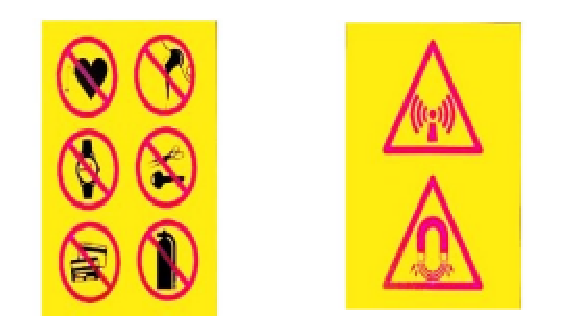
\includegraphics[width=0.7\textwidth]{seguridad_prohibidos}
   \caption{Señalamientos de seguridad para entornos de Resonancia Magnética: a) de izquierda a derecha y de arriba hacia abajo \textsc{No introducir marcapasos}, \textsc{Implantes}, \textsc{Relojes}, \textsc{Objetos ferromagnéticos}, \textsc{Tarjetas con banda magnética} y \textsc{Extintores}; b) de arriba hacia abajo, \textsc{Precaución: Radiofrecuencia} y \textsc{Magnetización}.}
 \label{fig:seguridad_prohibidos}
 \end{figg}
\end{figure}


